\documentclass{UTNetLab}

\title{TCP and Its Applications}
\newcommand\reference{
   S. Panwar, S. Mao, J.-dong Ryoo, and Y. Li, “TCP study,” in TCP/IP Essentials: A Lab-Based Approach, Cambridge: Cambridge University Press, 2004, pp. 111–133.
}

\begin{document}
	\section*{Objectives}
	\begin{itemize}
		\item TCP connection establishment and termination.
		\item TCP timers.
		\item TCP timeout and retransmission.
		\item TCP interactive data flow, using \textbf{telnet} as an example.
		\item TCP bulk data flow, using \textbf{socket} as a traffic generator.
		\item Further comparison of TCP and UDP.
		\item Tuning the TCP/IP kernel.
	\end{itemize}
	
	
\part{Exercises on TCP Connection Control}
    Like the previous lab, connect two hosts with one hub together (Figure~5.0) or use Figure~1.3 with two hosts.
    
\section{Telnet terminal}
   While \lstbash{wireshark} is running, execute: \lstbash[emph={h0,h1,netlab}]{telnet h1.netlab echo} on the \textit{h0} host, then type some text.
   
   Save the \lstbash{wireshark} output.
		
	\fcolorbox{blue}{lime!30}{{h\textsubscript{0}'s Wireshark}}
     \lstset{backgroundcolor=\color{lime!30}}
     \begin{lstlisting}
     Run wireshark on eth1, Filter: ip.addr == 128.238.61.100 && ip.addr == 128.238.61.101

     \end{lstlisting}  
    
	\fcolorbox{blue}{red!10}{{h\textsubscript{0}}'s \lstinline{Console}}
	\lstset{backgroundcolor=\color{red!10}}
	\begin{lstlisting}[emph={remote-host}]
	telnet 128.238.61.101 echo -e q
	\end{lstlisting}

	\textbf{Note:} We set the \textit{q} character as an \textit{escape} character. So, do not type q character. 
	
	At the end, you can close the telnet connection by typing \textit{q} character and run \textit{close} command.

\fcolorbox{blue}{red!10}{{h\textsubscript{0}}'s \lstinline{Console}}
\lstset{backgroundcolor=\color{red!10}}
\begin{lstlisting}
	q
	close
\end{lstlisting}
   
    \begin{report}
        \item Explain TCP connection establishment and termination using the \lstinline{wireshark} output.
        
        \item What were the announced MSS values for the two hosts?
        
        \item What happens if there is an intermediate network that has an MTU less than the MSS of each host?
    	See if the \texttt{DF}\footnote{Don't Fragment} flag was set in \lstinline{wireshark} output.
    
    	You can change interface \texttt{MTU} with below command:
	
		\fcolorbox{blue}{red!10}{{h\textsubscript{0}}'s Console}
		\lstset{backgroundcolor=\color{red!10}}	
		\begin{lstlisting}[emph=$eth]
sudo ifconfig eth1 mtu 68
		\end{lstlisting}
	
		\fcolorbox{blue}{red!10}{{h\textsubscript{1}}'s Console}
		\lstset{backgroundcolor=\color{red!10}}
		\begin{lstlisting}[emph=$eth]
sudo ifconfig eth1 mtu 68
		\end{lstlisting}

    \end{report}
    
\section{TCP vs UDP Connection Establishment}
    
    While \lstbash[emph={h0,h1,netlab}]{wireshark} is running, use \lstbash{socket}\footnote{Basic command is \lstbash{sock}. Use alternative \lstbash{socket} (linked to \lstbash{sock}).} to send a UDP datagram to the \textit{h1} host from the \textit{h0} machine:
    
    \fcolorbox{blue}{lime!30}{{h\textsubscript{0}'s Wireshark}}
     \lstset{backgroundcolor=\color{lime!30}}
     \begin{lstlisting}
     Run wireshark on eth1, Filter: ip.addr == 128.238.61.100 && ip.addr == 128.238.61.101

     \end{lstlisting}  
    
    \fcolorbox{blue}{red!10}{{h\textsubscript{0}}'s Console}
    \lstset{backgroundcolor=\color{red!10}}
    \begin{lstlisting}[emph={h0,h1,netlab}]
    socket -u -i -n1 128.238.61.101 8888
    \end{lstlisting}
    
    {Save} the \lstbash{wireshark} output for your lab report. \\
    Restart the above \lstbash{wireshark} capturing, execute \lstbash{socket} in the TCP mode:
    
    \fcolorbox{blue}{lime!30}{{h\textsubscript{0}'s Wireshark}}
     \lstset{backgroundcolor=\color{lime!30}}
     \begin{lstlisting}
     Run wireshark on eth1, Filter: ip.addr == 128.238.61.100 && ip.addr == 128.238.61.101

     \end{lstlisting}  
       
    \fcolorbox{blue}{red!10}{{h\textsubscript{0}}'s \lstinline{Console}}
    \lstset{backgroundcolor=\color{red!10}}
    \begin{lstlisting}[emph={h1,netlab}]
    socket -i -n1 128.238.61.101 8888
    \end{lstlisting}       
        
    {Save} the \lstbash{wireshark} output for your lab report.    
    
   \begin{report}
        \item Explain what happened in both the UDP and TCP cases.
                When a client requests a non-existing server, how do UDP and TCP handle this request, respectively?
    \end{report}

\part{Exercise on TCP Interactive Data Flow}
\section{Interactive Data Flow}
			
	While \lstinline{wireshark} captures the traffic between your machine and a remote machine, issue the following commands:
	
	\fcolorbox{blue}{lime!30}{{h\textsubscript{0}'s Wireshark}}
     \lstset{backgroundcolor=\color{lime!30}}
     \begin{lstlisting}
     Run wireshark on eth1

     \end{lstlisting}  
	
	\fcolorbox{blue}{red!10}{{h\textsubscript{0}}'s \lstinline{Console}}
	\lstset{backgroundcolor=\color{red!10}}
	\begin{lstlisting}[emph={h1,netlab}]
	telnet 128.238.61.101
	\end{lstlisting}

	Enter \lstinline[emph={netlab}]{"netlab"} as username and password for login in the remote host. After logging in to the host, type \lstinline{date} and press the {Enter} key.

    Now, in order to generate data faster than the round-trip time of a single byte to be sent and echoed, type any sequence of keys in the \lstinline{telnet} window very rapidly.\footnote{For example hold ``A'' key or write ``qwertyuiop'' in \lstinline{telnet} window.}

    {Save} the \lstinline{wireshark} output for your lab report.
    
    \begin{report}[{Answer the following questions, based upon the \lstinline{wireshark} output saved in the above exercise.}]
        \item What is a delayed acknowledgement?
            What is it used for?
        
        \item Can you see any delayed acknowledgements in your \lstinline{wireshark} output?

            If yes, explain the reason.
            Mark some of the lines with delayed acknowledgements, and submit the \lstinline{wireshark} output with your report.

            Explain how the delayed ACK timer operates from your \lstinline{wireshark} output.

            If you don’t see any delayed acknowledgements, explain the reason why none was observed.
        
        \item What is the \textit{Nagle}\footnote{Nagle Algorithm is a means of improving the efficiency of TCP/IP networks by reducing the number of packets that need to be sent over the network.} algorithm used for?

            From your \lstinline{wireshark} output, can you tell whether the \textit{Nagle} algorithm is enabled or not? Give the reason for your answer.

            From your \lstinline{wireshark} output for when you typed very rapidly, can you see any segment that contains more than one character going from your host to the remote machine?
            
            Now add link delay in the simulator \footnote{In PNETLab, \lstinline{right-click} on the link, select \lstinline{Quality} and set the link \lstinline{delay} to \textit{100 ms}} and do the same experiment again. Can you tell whether the Nagle algorithm is enabled or not? When you typed very rapidly, can you see any segment that contains more than one character going from your host to the remote machine?
    \end{report}

\part{Exercise on TCP Bulk Data Flow}
\section{IP Segment}
    Run \lstinline{wireshark} on your host by:
		
    \fcolorbox{blue}{lime!30}{{h\textsubscript{0}'s Wireshark}}
     \lstset{backgroundcolor=\color{lime!30}}
     \begin{lstlisting}
     Run wireshark on eth1, Filter: ip.addr == 128.238.61.100 && ip.addr == 128.238.61.101

     \end{lstlisting}  

    While \lstinline{wireshark} is running and capturing the packets between your machine and a remote machine, on the remote machine, which acts as the server, execute:

	\fcolorbox{blue}{red!10}{{h\textsubscript{1}}'s Console}
	\lstset{backgroundcolor=\color{red!10}}
	\begin{lstlisting}
	socket -i -s 7777
	\end{lstlisting}

    Then, on your machine's which acts as the client, execute:

	\fcolorbox{blue}{red!10}{{h\textsubscript{0}}'s \lstinline{Console}}
	\lstset{backgroundcolor=\color{red!10}}
	\begin{lstlisting}[emph={h1,netlab}]
	socket -i -n16 128.238.61.101 7777
	\end{lstlisting}
	
    Do the same experiment three times.

    Save all the \lstinline{wireshark} outputs for your lab report.
    
    \begin{report}
        \item Using one of three \lstinline{wireshark} outputs, explain the operation of TCP in terms of data segments and their acknowledgements.
                Does the number of data segments differ from that of their acknowledgements?

            Compare all the \lstinline{wireshark} outputs you saved.
            Discuss any differences among them, in terms of data segments and their acknowledgements.
        
        \item From the \lstinline{wireshark} output, how many different TCP flags can you see? Enumerate the flags and explain their meanings.

            How many different TCP options can you see?
            Explain their meanings.
    \end{report}

\part{Exercises on TCP Timers and Retransmission}
\section{Keepalive parameter}
Execute \lstbash{sysctl -A | grep keepalive} to display the default values of the TCP kernel parameters that are related to the TCP keepalive timer.
	
	\fcolorbox{blue}{red!10}{{h\textsubscript{0}}'s Console}
	\lstset{backgroundcolor=\color{red!10}}
	\begin{lstlisting}[emph={your-host, remote-host}]
	sysctl -A | grep keepalive
	\end{lstlisting}

    \begin{report}
        \item What is the default value of the TCP keepalive timer?
        
        \item What is the maximum number of TCP keepalive probes a host can send?
    \end{report}

\section{TCP Retransmission}
Run \lstinline{wireshark} on your host by:
		
    \fcolorbox{blue}{lime!30}{{h\textsubscript{0}'s Wireshark}}
     \lstset{backgroundcolor=\color{lime!30}}
     \begin{lstlisting}
     Run wireshark on eth1, Filter: ip.addr == 128.238.61.100 && ip.addr == 128.238.61.101

     \end{lstlisting}  
While \lstinline{wireshark}  is running to capture the packets between your host and a remote host, start a \lstinline{socket} server on the remote host,

	\fcolorbox{blue}{red!10}{{h\textsubscript{1}}'s Console}
	\lstset{backgroundcolor=\color{red!10}}
	\begin{lstlisting}
	socket -s 8888
	\end{lstlisting}
Then add link delay in the simulator\footnote{In PNETLab, \lstinline{right-click} on the link, select \lstinline{Quality} and set the link \lstinline{delay} to \textit{100 ms}} and execute the below command on your host's console,
	
	\fcolorbox{blue}{red!10}{{h\textsubscript{0}}'s \lstinline{Console}}
	\lstset{backgroundcolor=\color{red!10}}
	\begin{lstlisting}[emph={h1,netlab}]
	socket -i -n200 -p 100 128.238.61.101 8888
	\end{lstlisting}

While the sender is injecting data segments into the network, try to interrupt the connection by suspending the link between the hub and host \textit{h1}. For this purpose, \texttt{right-click} on the \textit{eth1} interface label of the host \textit{h1} and select \texttt{suspend} as shown in Figure \ref{p01}.

\begin{figure}[H]
    \centering
    {\selectlanguage{english}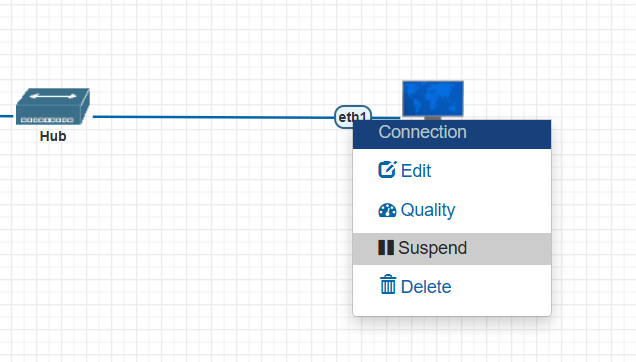
\includegraphics[scale=0.7]{img/1.png}}
    \caption{Right-click on the \textit{eth1} label}
    \label{p01}
\end{figure}

After observing several retransmissions, \textbf{reconnect the network by resuming the connection.} For this purpose, again \texttt{right-click} on the \textit{eth1} interface label of the host \textit{h1} and this time select \texttt{resume}.

When all data segments are sent, save the \lstinline{wireshark} output for the lab report.
    
    \begin{report}
        \item Submit the \lstinline{wireshark} output saved in this exercise.
        
        \item From the \lstinline{wireshark} output, identify when the cable was disconnected.
        
        \item Describe how the retransmission timer changes after sending each retransmitted packet, during the period when the cable was disconnected.
        
        \item Explain how the number of data segments that the sender transmits at once (before getting an ACK) changes after the connection is reestablished\footnote{Can see TCP \textbf{window scale} option and \textbf{RTT}}.
    \end{report}
    
\part{Other Exercises}
\section{Fragmentation}
    Run \lstinline{wireshark} on your host by:
		
	\fcolorbox{blue}{lime!30}{{h\textsubscript{0}'s Wireshark}}
     \lstset{backgroundcolor=\color{lime!30}}
     \begin{lstlisting}
     Run wireshark on eth1, Filter: ip.src == 128.238.61.100
     \end{lstlisting}  

    While \lstinline{wireshark} is running, execute the following command, which is similar to the command we used to find out the maximum size of a UDP datagram in the previous lab session (Chapter~5 of reference book),
	
	\fcolorbox{blue}{red!10}{{h\textsubscript{0}}'s \lstinline{Console}}
	\lstset{backgroundcolor=\color{red!10}}
	\begin{lstlisting}[emph={n, h1,netlab}]
	socket -i -n1 -w 70080 128.238.61.101 echo
    \end{lstlisting}
    
   \textbf{Note:}  \textit{70080} is larger than the maximum UDP datagram size we found in previous lab session.



    \begin{report}
        \item Did you observe any IP fragmentation?
            
        \item If IP fragmentation did not occur this time, how do you explain this compared to what you observed in previous lab session for UDP packets?
    \end{report}

\section{Linux TCP/IP Kernel Parameter}
    Study the manual page of \lstinline{/sbin/sysctl}.
    
    \fcolorbox{blue}{red!10}{{h\textsubscript{0}}'s Console}
	\lstset{backgroundcolor=\color{red!10}}
	\begin{lstlisting}
	man /sbin/sysctl
	\end{lstlisting}
	
    Examine the default values of some TCP/IP configuration parameters that you might be interested in.
    
    Examine the configuration files in the \path{/proc/sys/net/ipv4} directory.    

	\fcolorbox{blue}{red!10}{{h\textsubscript{0}}'s Console}
	\lstset{backgroundcolor=\color{red!10}}
	\begin{lstlisting}
	cd /proc/sys/net/ipv4
	\end{lstlisting}
	

    
   {Note:} You can see the directory files and folders by:

	\fcolorbox{blue}{red!10}{{h\textsubscript{0}}'s Console}
	\lstset{backgroundcolor=\color{red!10}}
	\begin{lstlisting}
	ls
	\end{lstlisting}
	
	Also, you can see files contents with the below command:

	\fcolorbox{blue}{red!10}{{h\textsubscript{0}}'s Console}
	\lstset{backgroundcolor=\color{red!10}}
	\begin{lstlisting}[emph={file-name}]
	cat file-name
	\end{lstlisting}

    \begin{report}
        \item Explain what is \lstinline{sysctl} command for?
            
        \item Explain two arbitrary TCP/IP configuration parameters.
                What is their default values?
            
        \item Name two arbitrary file in the \path{/proc/sys/net/ipv4} directory.
                What is their content?
    \end{report}

\end{document}